\documentclass[11pt,border=5pt]{standalone}
\usepackage{fontspec}
\setmainfont{cmunrm.otf}[BoldFont=cmunbx.otf,ItalicFont=cmunti.otf,BoldItalicFont=cmunbi.otf]
\usepackage{amsmath}
\usepackage{unicode-math}
\setmathfont{NewCMMath-Regular.otf}
\usepackage{tikz}
\usetikzlibrary{arrows.meta,patterns,angles,quotes}
\begin{document}
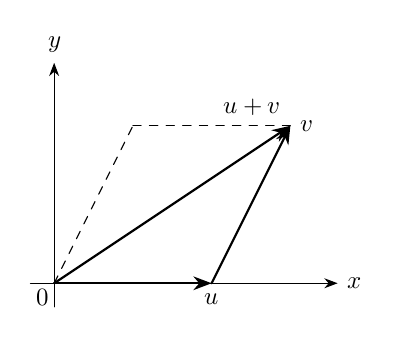
\begin{tikzpicture}[>=Stealth,font=\small,line cap=round,line join=round]
\draw[->,thin] (-0.3,0) -- (3.6,0) node[right] {$x$};
\draw[->,thin] (0,-0.3) -- (0,2.8) node[above] {$y$};
\node at (-0.14,-0.18) {$0$};
\draw[->,thick] (0,0) -- (2,0) node[below] {$u$};
\draw[->,thick] (2,0) -- (3,2) node[right] {$v$};
\draw[->,thick] (0,0) -- (3,2) node[above left] {$u+v$};
\draw[dashed] (0,0) -- (1,2);
\draw[dashed] (1,2) -- (3,2);

\end{tikzpicture}
\end{document}
